
\begin{figure}[t]
	\centering
	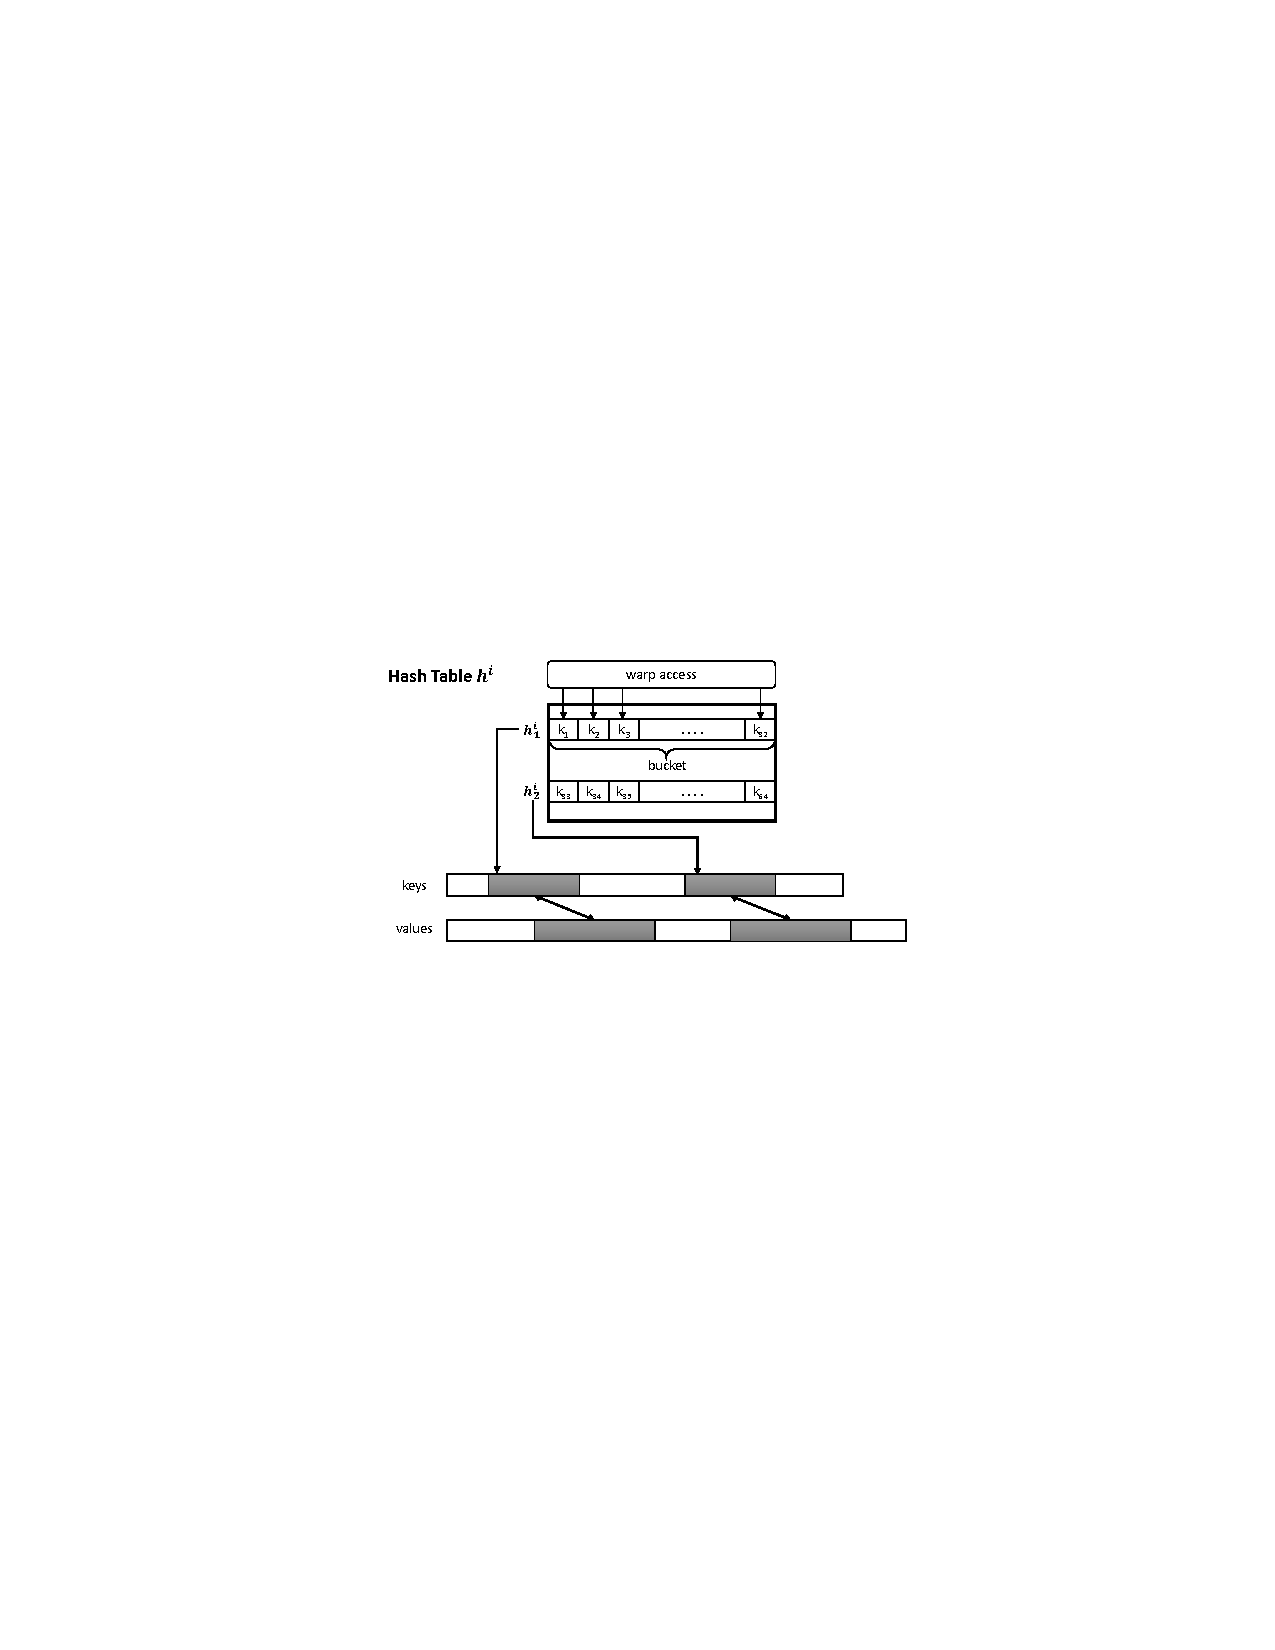
\includegraphics[width=0.45\textwidth]{fig/Hashtable.pdf}
	\caption{The hash table structure}
	\label{fig:hashtable}
\end{figure}

\section{Voter-based GPU Cuckoo Hash}\label{sec:vot}
In this section, we first present a overview of the hash table structure and pinpoint a number of important design objectives in Section~\ref{sec:vot:has}.
Subsequently, in Section~\ref{sec:vot:con}, we give details on how to perform updates with the \emph{voter} coordination, i.e., \formal{find}, \formal{insert} and \formal{delete}, for the case where hash table resizing is not required. 
We leave how to handle the fully dynamic scenario in Section~\ref{sec:dyn} for further discussions. 

\subsection{Hash Table Structure}\label{sec:vot:has}
Adopted from cuckoo hashing \cite{}, we build $d$ hash tables with $d$ unique hash functions: $h^1,h^2,\ldots,h^d$. 
In this work, we use a set of simple universal hash function such as $h^i(k) = (a_i\cdot k + b_i \mod p) \mod |h^i|$.
$a_i,b_i$ are random integers, $p$ is a large prime.
There are three major advantages for adopting cuckoo hashing on GPUs. 
First, it avoids chaining by inserting the elements into alternative locations if collision happens. As discussed in Section~\ref{sec:rel}, 
chaining present several issues which are not friendly to the GPU architecture.  
Second, to lookup a KV pair, one only needs to search $d$ locations specified by $d$ unique hash functions. 
Thus, the data could be stored contiguously in the same location and thus enable the preferred coalesced memory access. 
Third, cuckoo hashing can maintain high filled factor, which is ideal for memory saving in the dynamic scenario. 
For $d=3$, cuckoo hashing achieves over $90\%$ filled factor and still process \formal{insert} operations efficiently \cite{fotakis2005space}.

Figure~\ref{fig:hashtable} depicts the design of a single hash table $h^i$ on GPUs. 
Assuming the keys are 4-byte integers. A bucket of 32 keys, which are all hashed to the same value $h^i_j$, are stored consecutively in the memory. 
The design of buckets maximizes the utilization of memory bandwidth in GPUs. 
Since the cache line size is 128 bytes, only a single access is required when one warp is assigned to access a bucket. 
The values associated with the keys in the same bucket are also stored consecutively but in a separate array.   
In other words, we use two arrays to store the keys and the values respectively.
The values could take much larger memory space than the keys. 
Thus, storing keys and values separately avoid the overhead of memory access when accessing the values are not necessary, 
e.g., finding a nonexistent KV pair or deleting a KV pair. 

For keys having size larger than 4 bytes, a simple strategy is to store less KV pairs in a basket. For example, if the keys are 8-types, then a basket can accommodate 16 KV pairs. In the worst case, a key taking 128 bytes occupy one basket alone, which is unnecessary large in practice.


\begin{algorithm}[t]
	\begin{algorithmic}[1]
		\State $found \gets \emptyset$
		\For{$i=0,\ldots,d-1$}
		\State $loc \gets h^i(k)$
		\State $found \gets ballot(loc[l].key == k)$
		\If{$found \neq \emptyset$}
		\State \Return $loc[l]$
		\EndIf
		\EndFor
		\State \Return false
	\end{algorithmic}
	\caption{\textbf{Find}(lane $l$, warp $wid$, key $k$)}\label{algo:find}
\end{algorithm}

\subsection{Parallel Hash Table Operations}\label{sec:vot:con}
In the reminder of this session, we discuss how to utilize GPUs' threads to execute hash table operations in parallel.
Following existing works \cite{alcantara2009real,zhang2015mega,breslow2016horton}, we assume the \formal{find}, \formal{insert} and \formal{delete} operations are batched and each batch only contains one type of operations. A batch with mixed type of operations can also be supported but the semantic is ambiguous. 



\vspace{1mm}\noindent\textbf{Find.} It is relative straightforward to parallelize \formal{find} operations since only read access is required. 
Given a batch of size $m$, we launch $w$ warps in total (which means launching $32w$ threads in total) and each warp is responsible for $\floor{\frac{m}{w}}$ \formal{find} operations. To locate a KV, we need to hash the key with $d$ hash functions and look for the corresponding locations. 
Algorithm~\ref{algo:find} presents the pseudo code for a KV lookup by a warp. 
First, the bucket of the $i$th hash table is located, i.e., $loc_i$.
Then, each thread in the warp (a thread lane $l$) simultaneously searches the key and the ballot function return the lane for which the key is found.

\begin{figure}[t]
	\hspace{-3em}
	\begin{minipage}{0.5\linewidth}
		\label{fig:atomicCAS}
		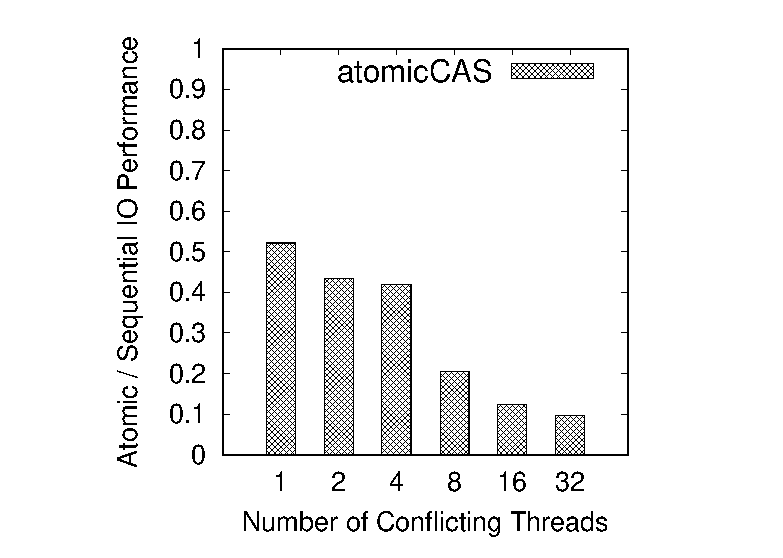
\includegraphics[width=5.3cm]{exp/atomic/atomicCAS.eps}
	\end{minipage}
	\hspace{-1em}
	\begin{minipage}{0.5\linewidth}
		\label{fig:atomicExch}
		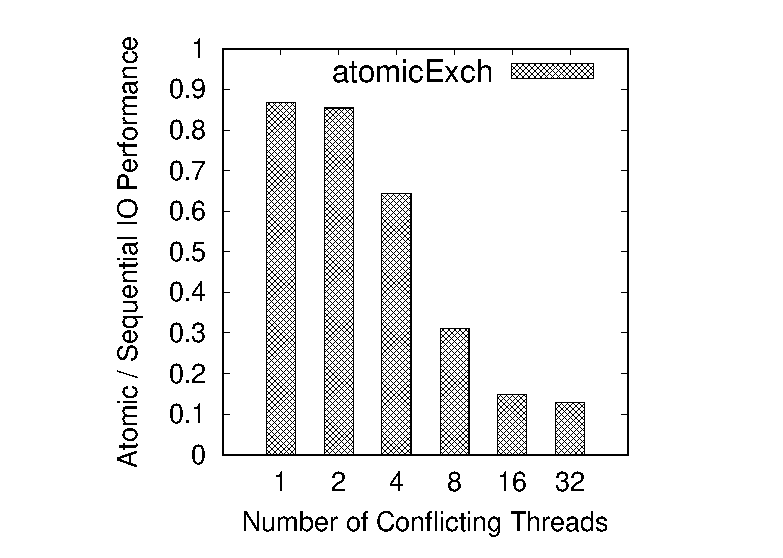
\includegraphics[width=5.3cm]{exp/atomic/atomicExch.eps}
	\end{minipage}
	\caption{The performance of atomic operations for varying number of conflicts}
	\label{fig:atomic}
\end{figure}

\begin{algorithm}[t]
	\begin{algorithmic}[1]
		\State $active \gets 1$	\label{algo:insert:active:start}
		\While{true}
		\State $l' \gets ballot(active == 1)$ \label{algo:insert:vote:start}
		\If{$l'$ is invalid}
		\State break \label{algo:insert:active:end}
		\EndIf
		\State $[(k',v'),i'] \gets broadcast(l')$ \label{algo:insert:lock:start}
		\State $loc = h^{i'}(k')$
		\If{$l' == l$}
		\State $success \gets lock(loc)$ \label{algo:insert:lock:end}
		\EndIf
		\If{$broadcast(success,l') ==$ failure}
		\State continue					\label{algo:insert:vote:end}
		\EndIf
		\State $l^* \gets ballot(loc[l].key == k' || loc[l].key ==\emptyset)$ \label{algo:insert:write:start}
		\If{$l^*$ is valid and $l' == l$}
		\State $loc[l^*].(key,val) \gets (k',v')$
		\State $unlock(loc)$
		\State $active \gets 0$;
		\State continue			\label{algo:insert:write:end}
		\EndIf
		\State $l^* \gets ballot(loc[l].key \neq \emptyset)$
		\If{$l^*$ is valid and $l' == l$}
		\State $swap(loc[l^*].(key,val),(k',v'))$
		\State $unlock(loc)$
		\State $i \gets i+1$ \label{algo:insert:loop:end}
		\EndIf
		\EndWhile
	\end{algorithmic}
	\caption{\textbf{Insert}(lane $l$, warp $wid$, kv $(k,v)$, table $i$)}\label{algo:insert}
\end{algorithm}

\vspace{1mm}\noindent\textbf{Insert.} Contention occurs when multiple \formal{insert} operations target at the same bucket. 
There are two conflicting objectives for resolving the contention. On one hand, we want to utilize the warp-centric approach to access a bucket.
On the other hand, a warp requires a mutex when updating a bucket to avoid corruption, and the locking is expensive on GPUs.  
In the literature, it is a common practice to use atomic operations for implementing a mutex under the warp-centric approach \cite{zhang2015mega}. 
In particular, we can still invoke a warp to insert a KV pair. The warp is required to acquire a lock before updating the corresponding bucket. 
The warp will keep trying to acquire the lock before successfully obtain the control. 
There are two drawbacks for this direct warp-centric approach. 
First, the conflicting warps are spinning while locking, thus wasting computing resources.
Second, although atomic operations are supported by recent GPU architectures natively, 
they become costly when the number of atomic operations issuing at the same location increases. 
In Figure~\ref{fig:atomic}, we show the profiling statistics for two atomic operations which are often used to lock and unlock a mutex: atomicCAS and atomicExch respectively. 
We compare the throughputs of the atomic operations vs. an equivalent amount of sequential device memory IOs (coalesced) and present the trend for varying the number of conflicting atomic operations. It is apparent that the atomic performance has seriously degraded for a larger number of conflicts. 
Thus, it will be expensive for the direct warp-centric approach in the contention critical cases. 
Imaging one wants to track the number of retweets posted to active twitter accounts in the current month, via storing the twitter ID and the obtained retweet counts as KV pairs. In this particular scenario, certain twitter celerities could receive thousands of retweets in a very short period. 
This triggers the same twitter ID gets updated frequently and a serious number of conflicts would happen. 

To alleviate the cost of spinning, we propose the voter-coordination scheme. 
We assign an \formal{insert} to a thread rather than using a warp to handle the operation. Before submitting a locking request and updating the corresponding bucket, the thread will participate in a vote among the threads in the same warp. 
The winner thread $l$ becomes the leader of the warp and takes control. Subsequent, the warp inspects the bucket and insert the KV for $l$ if there are spaces left, upon $l$ successfully obtaining the lock.
If $l$ fails to get the lock, the warp revotes another leader to avoid locking on the same bucket.
Compared with locking on atomic operations, the cost of warp voting is almost negligible since it is heavily optimized in the GPU architecture.  


Parallel insertion with the voter coordination scheme is presented in Algorithm~\ref{algo:insert}.
The pseudo code demonstrates how a thread (with lane $l$) from warp $wid$ inserts a KV $(k,v)$ to the $i$th hash table. 
The warp will first propose a vote among active threads and the process will terminate if all threads finish their tasks (lines~\ref{algo:insert:active:start}-\ref{algo:insert:active:end}).  
This achieves better resource utilization since no thread will be idle when one of the threads in the same warp is active.  
The leader $l'$ then broadcasts its KV pair $(k',v')$ as well as the hash table index $i'$ to the warp and tries to lock the inserting bucket (lines~\ref{algo:insert:lock:start}-\ref{algo:insert:lock:end}). 
The broadcast function ensures all threads in the warp receive the locking result and the warp revotes if $l'$ fails to obtain the lock.
Otherwise, the warp follows $l'$ and proceeds to update the bucket for $(k',v')$ with a warp-centric approach similar to \formal{find}.
Once a thread finds $k'$ or an empty space in the bucket, $l'$ will add or update with $(k',v')$ (lines~\ref{algo:insert:write:start}-\ref{algo:insert:write:end}).
Otherwise there is no space left, $l'$ swaps $(k',v')$ with a random KV in the bucket and inserts the evicted KV to hash table $i+1$ in the next round. 
In summary, each iteration of the loop presented in Algorithm~\ref{algo:insert} issues $1$ atomic operation and at most $1$ device memory read/write (lines~\ref{algo:insert:vote:start}-\ref{algo:insert:loop:end}).  

Note that we have yet covered how to choose the hash table index $i$ for each insertion (Algorithm~\ref{algo:insert}). Additional number of conflicts would happen if all threads attempting to insert to the same table. For the flow of presentation, we leave the discussion to Section~\ref{sec:dyn} since choosing the hash table is more coherent to the load balancing problem for resizing hash tables. Moreover, a careful reader would find that the insertion process could lead to multiple appearances of the same key in different hash tables. To fill this gap, one can attach a timestamp to the insertion batch.
Hence, the \formal{find} operation is required to scan all $d$ buckets of the same key and extracts the one with the latest timestamp.

\begin{figure}[t]
	\centering
	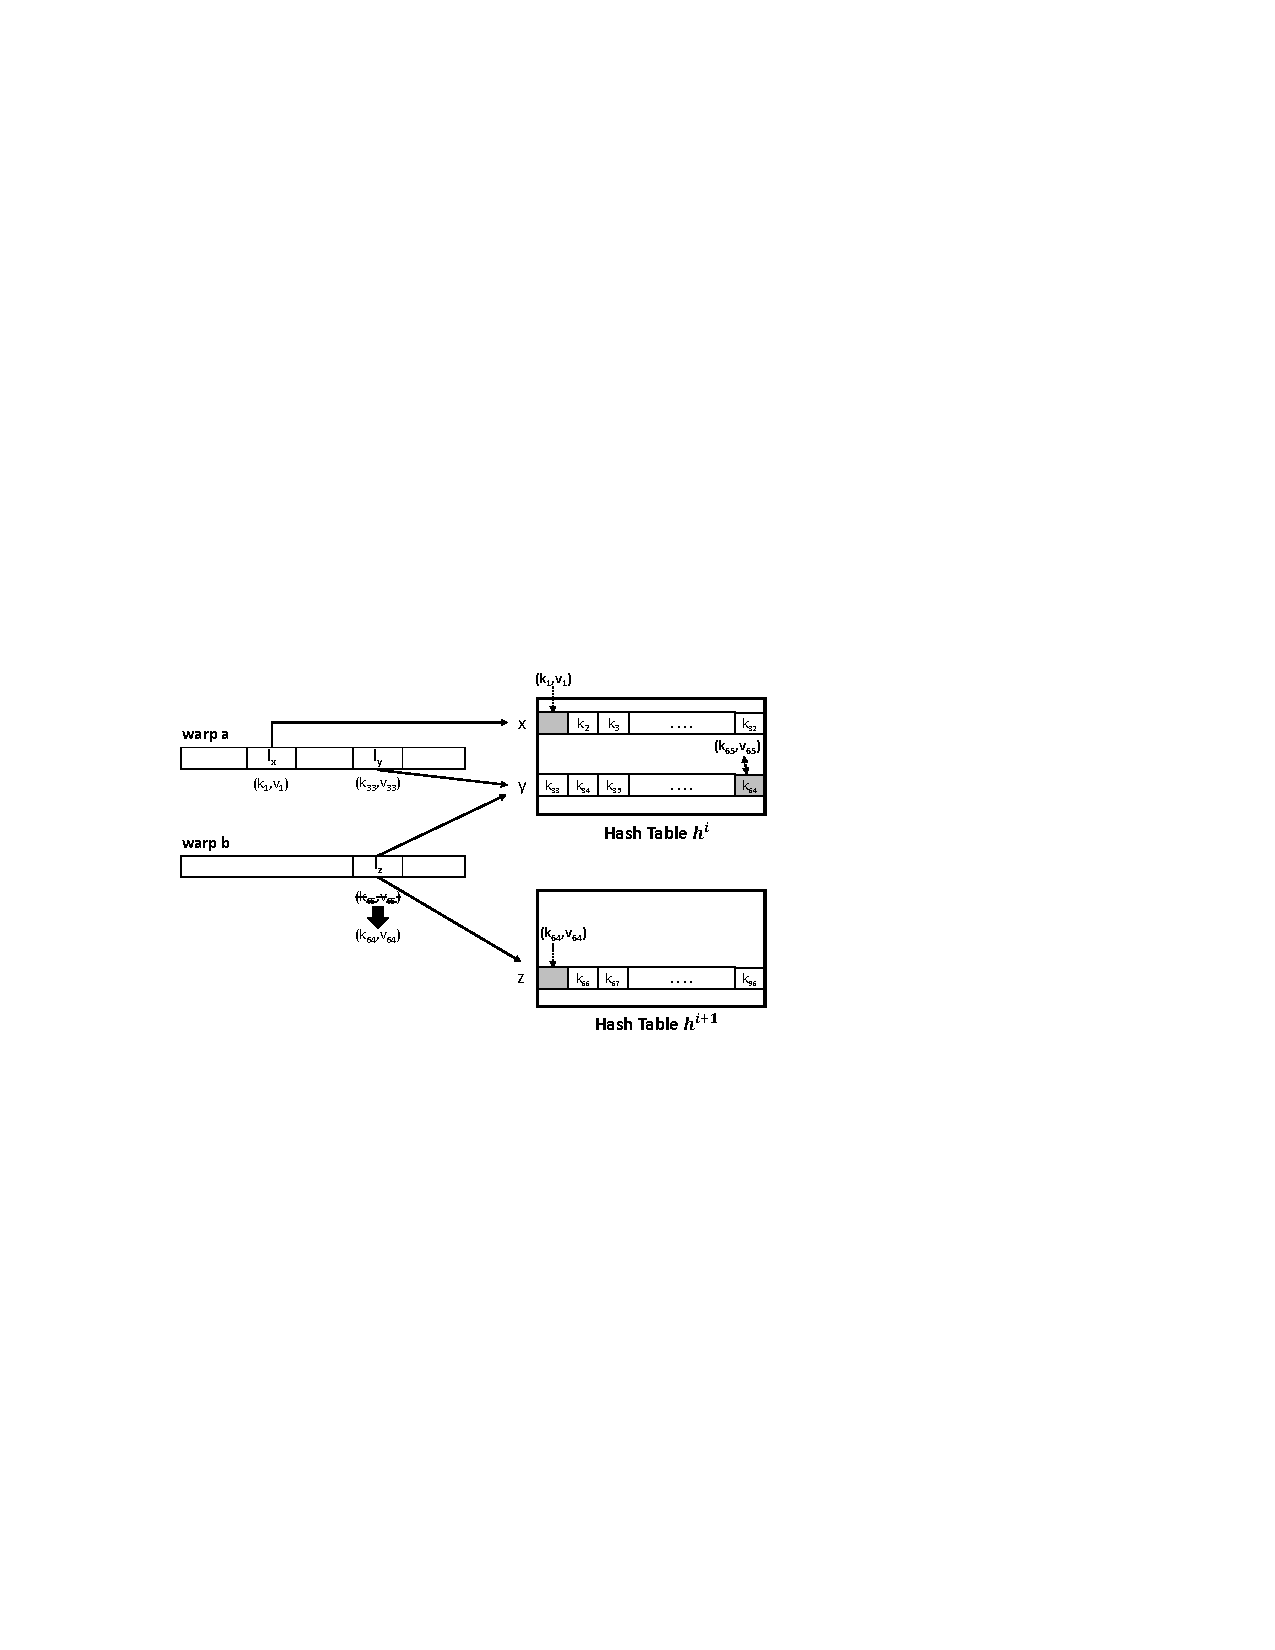
\includegraphics[width=0.45\textwidth]{fig/Voter.pdf}
	\caption{Example for parallel insertions}
	\label{fig:voter}
\end{figure}

We give the following example to demonstrate the parallel insertion process.
\begin{example}
	In Figure~\ref{fig:voter}, we visualize the scenario for three threads: $l_x$, $l_y$, $l_z$ from warp $a$ and warp $b$, inserting KV pairs $(k_1,v_1)$,$(k_{33},v_{33})$,$(k_{65},v_{65})$ independently. 
	Suppose $l_y$ and $l_z$ become the leaders of warp $a$ and $b$ respectively. Both threads will compete for the bucket $y$ and $l_z$ wins the battle. 
	$l_z$ will then leads warp $b$ to inspect the bucket and evict $(k_{64},v_{64})$ by replacing with $(k_{65},v_{65})$. 
	In the meanwhile, $l_y$ does not lock on bucket $y$ and joins the new leader $l_x$ voted in warp $a$. 
	$l_x$ locks bucket $x$ and inserts $(k_1,v_1)$ in place. Subsequently, $l_y$ may get back the control of warp $a$ and update $k_{33}$ with $(k_{33},v_{33})$ at bucket $y$. In parallel, $l_z$ locks bucket $z$ and inserts the evicted KV $(k_{64},v_{64})$ into the empty space. 
\end{example}

\vspace{1mm}\noindent\textbf{Delete.} The \formal{delete} operation, in contrast to \formal{insert}, does not require locking with a warp-centric approach. 
Similar to \formal{find}, we assign a warp to process a key $k$ on deletion. The warp iterates through the buckets among all $d$ hash tables that could possibly contain $k$. Each thread lane in the warp is responsible for inspecting one position in a bucket independently, and only erase the key if $k$ is found, 
thus causes no contention.

%\begin{algorithm}[t]
%	\begin{algorithmic}[1]
%		\For{$i=1,\ldots,d$}
%			\State $loc \gets h^i(k)$
%			\State $found \gets (loc[l].key == k)$
%			\If{$found$}
%				\State $loc[l].key \gets \emptyset$
%			\EndIf
%		\EndFor
%	\end{algorithmic}
%	\caption{\textbf{Delete}(lane $l$, warp $wid$, key $k$)}\label{algo:delete}
%\end{algorithm}


\vspace{1mm}\noindent\textbf{Complexity.}
Since a \formal{find}, \formal{insert} and \formal{delete} operation is independently executed by a thread. 
The analysis of a single thread complexity is the same as the sequential version of cuckoo hashing \cite{pagh2004cuckoo}: $O(1)$ worst case complexity for \formal{find} and \formal{delete}, $O(1)$ expected time for \formal{insert} for the case of 2 hash tables. 
It has been pointed out that analyzing the theoretical upper bound complexity of insertion in $d \geq 3$ hash tables is very difficult \cite{alcantara2009real}.  
Nevertheless, empirical results have shown that increasing the number of tables leads to better insertion performance, see our experiments in Section~\ref{sec:exp}.
Thus, we assume the complexity for inserting to $d$ hash tables is the same as that of $2$ has tables, as long as $d$ keeps constant.  

We then analyze the number of possible thread conflicts. Assuming we launch $m$ threads in parallel, each of them is assigned to an unique key, and the total number of unique buckets is $H=\sum_{i=1}^d|h^i|$. For \formal{find} and \formal{delete}, there is no conflict at all. 
For \formal{insert}, computing the expected number of conflicting buckets resembles the \emph{balls and bins} problem \cite{raab1998balls}, which is $O(\binom{m}{2}/H)$. 
Given GPUs have a large number of threads, there could be a significant amount of conflicts. Thus, we propose the voter coordination scheme to reduce the cost of spinning on locks. Note that the analysis is done for the cases where the key to update is unique. More conflicts could occur in reality when the same key is updated in parallel. 